\documentclass[12pt, letterpaper]{article}
\usepackage[margin=1.0in]{geometry}
\usepackage{amsmath}
\usepackage{amssymb}
\usepackage{fancyhdr}
\usepackage{pgfplots}
\usepackage{physics}
\usepackage{wrapfig}
\usepackage{hyperref}
\usepackage{multirow}

\pgfplotsset{compat=1.16}


\renewcommand{\thesubsection}{\thesection\Alph{subsection}}


\title{Particle Physics PS1}
\author{Joe Crowley}
\date{October 2020}

\pagestyle{fancy}
\renewcommand{\headrulewidth}{0pt}
\renewcommand{\footrulewidth}{0pt}

\fancyhf{}
\rhead{
Joe Crowley \\
Physics 225 \\
Problem Set 1
}
\rfoot{Page \thepage}

\begin{document}  

\section{CERN and the World Wide Web}
\textit{Do some research to learn about the origin of the World Wide Web, and write a paragraph or two discussing the early history of the Web. Try to address the following questions. How was the Web developed? Can you find text for the initial proposal? Who wrote it? What was the Web's initial purpose and what was the first Web site? What is the difference between the Web and the Internet? Be sure to check out the photo that I posted to GS.}\\

The web was developed over a period of nearly 20 years, from the original ``Data Communications" at CERN to the first website on W3. The original proposal for W3 was by Tim Berners-Lee in 1989. The first website was info.cern.ch, hosted on Tim Berners-Lee's NeXTcomputer. It was actually an info page about the world wide web. Very meta. The Internet is the graph of connections, and the Web is the information stored on the internet. I've seen that view in person! I even saw Tim Berners-Lee's original paper! I really liked this summary by Ben Segal from 1995: \href{http://ben.web.cern.ch/ben/TCPHIST.html}{http://ben.web.cern.ch/ben/TCPHIST.html}

\section{Decay modes of the Z boson}
\textit{This problem is to give you some practice using the Particle Data Book. Use the pdgLive or another version of the listings to answer the following simple questions. Important note: this is a list of experimental measurements, not theoretical predictions!}

\subsection{}
\textit{Make a short table listing the decay branching fraction of the $Z$ boson for which significant non-zero results have been obtained. (That is, you may ignore that ones with just an upper limit listed. ) Be sure to include $Z \rightarrow e^{+} e^{-}, Z \rightarrow \mu^{+} \mu^{-}, Z \rightarrow \tau^{+} \tau^{-}, Z \rightarrow$ invisible, $Z \rightarrow c \bar{c}, Z \rightarrow b \bar{b} .$ You
don't need to list the decay modes that involve specific hadrons, but you may if you want to.}\\

\begin{center}
\begin{tabular}{ |c||c| } 
\hline \hline
 Z Decay                  & $\frac{\Gamma_i}{\Gamma} \left(\%\right)$\\
 \hline \hline
    ${e^{+} e^{-}}$             & $3.3632 \pm 0.0042$\\
    $\mu^+ \mu^-$              & $3.3662 \pm 0.0066$\\
    $\tau^{+} \tau^-$              & $3.3696 \pm 0.0083$\\
    $\text { invisible }$              & $20.000 \pm 0.055$\\
    $C \bar{C}$                 & $12.03 \pm 0.21$\\
    $b \bar{b}$             & $15.12 \pm 0.05$\\
\hline \hline
\end{tabular}
\end{center}

\subsection{}
\textit{What do you think ``invisible" means in this listing? Are there any particles in the standard model (SM) that would be invisible experimentally?}\\

Invisible decay modes are decays that don't deposit a measurable amount of energy in the detector. $\nu_{\ell}$’s would be invisible experimentally, only found by ``missing momentum”.

\subsection{}
\textit{Do you observe any interesting patterns in the $Z$ boson branching fractions? These don't have to be fancy - just basic observations. For example, which decay modes have the largest branching fractions? Which modes are essentially the same? Do all modes to $q \bar{q}$ final states have the same branching fraction?}\\

The dilepton decay modes have a branching fraction that is approximately independent of flavour. The highest branchins fractions ar for hadronic decays.


\subsection{}
\textit{What are the mass, total decay width $(\Gamma),$ and spin of the $Z$ boson? How does the mass of the $Z$ boson compare to that of the proton? (When comparing two quantities that are very different in magnitude, it is usually best to compute their ratio, with the larger quantity in the denominator.)}\\

$$
M_{Z}=91.1876 \pm 0.0021\, \mathrm{GeV} \sim 90 m_p
$$
$$
\Gamma_{Z}=2.4952 \pm 0.0023\, \mathrm { GeV }
$$

\section{Indirect determination of a particle's lifetime from the spread in its mass values.} 
\textit{ $A$ quantum state with a finite (non-infinite) lifetime is not a true
energy eigenstate: it has a spread of energies! For a sample of particles with nominal mass $m$ (the rest frame energy), this implies that the mean liftime is related to the spread of observed mass values $\Gamma$ by $\tau=\frac{\hbar} { \Gamma}$. Later, we will derive the expression for the distribution of mass values, called the Breit-Wigner formula. Experimentally, $\Gamma$ can be measured from the full width at half maximum of the observed mass distribution, as long as the detector's mass resolution is good enough.}

\subsection{}
\textit{Look up the full width of the $Z$ boson and use it to compute its mean lifetime. A key point is that from the observed spread in masses of a sample of $Z$ bosons, one can measure $\Gamma_{Z}$ and thus infer the $Z$ lifetime, even though it is impossible to directly measure a lifetime that short!}

$$
\tau=\frac{\hbar}{\Gamma}
$$
$$
\Gamma_{z}=2.4952 \pm 0.0023 \text { GeV }
$$
$$
\tau_{z}=\frac{0.066 \operatorname{GeV} 10^{-23}\, \mathrm{s}}{2.4952 \,\mathrm{GeV}}
$$
$$\boxed{
\tau_{z}=2.6^{451} \times 10^{-25} \mathrm{s}}
$$

\subsection{}
\textit{Look up the lower limit on the mean lifetime of the proton. What limit does this result place on the full width $\Gamma$ of the proton mass distribution?}

$$
\tau_p > 2.1 \times 10^{29} \text { years } 
$$
$$
\frac{\hbar}{\Gamma_p}>2.1 \times 10^{24} \text { years }
$$
$$
\Gamma_{p}<\frac{h}{2.1\times10^{2 0} \text { years }}
$$
$$\boxed{
\Gamma_{p}<9.9 \times 10^{-62} \mathrm{GeV}}
$$

\subsection{}
\textit{Explain why it is not crazy to establish experimentally that a particle's lifetime is much greater than the age of the universe.}

If there are 0 decays observed with such a large quantity of protons, perhaps its decay width tends toward 0.

\subsection{}
\textit{The $\rho$ meson is a rather ``broad" particle, meaning that its width $\Gamma$ is substantial compared to its mean mass. Look up the $\rho$ in the RPP and compute $\Gamma / M .$ Note that the Particle Data Book does not distinguish among the three charge states of the $\rho: \rho^{\pm}$ and $\rho^{0} .$ This is because they all decay in the essentially the same way. This is not the case for the $\pi^{\pm}$ and $\pi^{0}$ at all! This is an example where it can be a bit tricky to read the information. If you have questions about it, feel free to ask me.}
$$
\frac{\Gamma_{\rho}}{M_{\rho}}=\frac{149.1\, \mathrm{MeV}}{775.26 \mathrm{MeV}}\,
$$
$$
\frac{\Gamma_{\rho}}{M_{\rho}}\approx19.2 \%
$$

\section{The electromagnetic coupling and the fine structure constant}
\textit{H-atom binding energy. The fine structure constant is essentially just the square of the charge of the electron, measured in appropriate units. As such, it is a fundamental constant that characterizes the strength of the $EM$ interaction.}

\subsection{}
\textit{The fine-structure constant $\alpha \simeq \frac{1}{137}$ is dimensionless, so you can use any consistent set of units to compute it. Compute $\alpha$ using SI units using the formula $\alpha=e^{2} /\left(4 \pi \epsilon_{0} \hbar c\right) .$ How close is $\alpha$ to $\frac{1}{137} ?$ When comparing two numbers that are very similar, the best approach is to compute a relative quantity like $(\alpha-1 / 137) / \alpha,$ not just the absolute difference. By the way, there is no magic to the number $1 / 137-$ it's just a cool thing. In fact, we will see that this is a ``running coupling constant," whose value changes slightly with energy according to a well-defined law.}
$$
\alpha_{E M}=\frac{e^{2}}{4 \pi \varepsilon_{0}\hbar C}
$$
$$
\approx 0.00729735257
$$
$$
\boxed{
\frac{\left|\alpha_{EM}-\frac{1}{137}\right|}{\alpha} \cdot 100 \%=0.02 \%}
$$

\subsection{}
\textit{Go to the Particle Data Group home page. Under Reviews, Tables, and Plots, find the article on the Electroweak Model and Constraints on New
Physics. This is a bit advanced for now, but read it anyway and write one paragraph on something that you find interesting in it.}

This is the first time I’m seeing perturbative QFT calculations of the masses, I am mostly used to seeing the experimental data and plots. I recognized some of the involved quantities such as weak mixing angle, I had seen that in the CERN summer student lectures and feel like I have much more background to understand these calculations. I particularly was interested in the calculation of the $\tau$ lifetime, because I have research experience writing simulations of upward $\tau$ decays for the ANITA experiment. 

\subsection{}
\textit{The energy levels of the H-atom are given by $E_{n}=-\frac{1}{2} m_{e} c^{2} \alpha^{2} \frac{1}{n^{2}},$ where $n$ is a positive integer. Compute the energy of the $n=1$ level in eV. To do this very quickly, start from the value of $m_{e} c^{2}$ in $\mathrm{eV},$ do not use joules!!!!!!}
$$
E_1=-\frac{1}{2} m_{e} c^{2} \alpha^{2}
$$
$$\boxed{
E_{1}=-13.6 \mathrm{eV}
}
$$

\subsection{}
\textit{The answer to the previous question is a negative number. Use this value to express the mass of the $H$ -atom in terms of the mass of $m_{p}$ and $m_{e}$ and the number you just computed, which is the binding energy for the $n=1$ (ground) state. (You might also ponder the question of why the binding energy is a negative quantity and whether this is the case for all systems.)}

Binding energy is negative because it represents the amount of energy required for an $e^-$ to ``escape'' the H atom.
$$
m_{\mathrm{H \, atom}}=m_{p}+m_{e}-E_{1}
$$
$$\boxed{
m_{\mathrm{H \, atom}}\approx 0.938783 \frac{\mathrm{GeV}}{c^{2}}
}
$$

\subsection{}
\textit{The velocity of an electron in an H-atom is roughly $v=\alpha c,$ where $c$ is the speed of light. What is the speed of the electron in $\mathrm{m} \mathrm{s}^{-1} ?$ Would you describe the H-atom as a highly relativistic, non-relativistic, or a weakly relativistic system?}

$$
v=\alpha c 
$$
$$
v=2.18769 \times 10^{6} \frac{m}{s}
$$

The 1s electron in hydrogen is weakly relativistic because 
$$
\beta \sim 0.01. 
$$

\subsection{}
\textit{Why is the fine-structure constant called the fine-structure constant? Look this up in your quantum mechanics book. Make a table listing the different contributions to the ``fine structure" in the H-atom. You don't need to derive anything, just write down the formulas for these energies and state what effects they correspond to. Hint: one of them is a relativistic correction. In summary, the term ``fine-structure constant" is historical,
and the quantity has a much greater relevance than $H$ -atom perturbation theory: it provides a dimensionless way to measure the charge of the electron. Because $\alpha<<1,$ it can be used in perturbation theory expansions for calculating a large number of processes in quantum electrodynamics.}


Perturbation theory! The H-atom wavefunction and interaction Hamiltonian includes the spin of the e, spin of the nucleus, and interactions between them and external fields.

\underline{Relativistic correction:}
$$
H_{r}^{\prime}=-\frac{p^{4}}{8 m^{3} c^{2}}
$$

\underline{Spin-Orbit correction:}
$$
H_{\mathrm{so}}^{\prime}=\left(\frac{e^{2}}{8 \pi \epsilon_{0}}\right) \frac{1}{m^{2} c^{2} r^{3}} \mathbf{S} \cdot \mathbf{L}
$$

\underline{Zeeman correction:}
$$
H_{Z}^{\prime}=\frac{e}{2 m}(\mathbf{L}+2 \mathbf{S}) \cdot \mathbf{B}_{\mathrm{ext}}
$$

\underline{Hyperfine correction:}
$$
H_{\mathrm{hf}}^{\prime}=\frac{\mu_{0} g_{p} e^{2}}{8 \pi m_{p} m_{e}} \frac{\left[3\left(\mathbf{S}_{p} \cdot \hat{r}\right)\left(\mathbf{S}_{e} \cdot \hat{r}\right)-\mathbf{S}_{p} \cdot \mathbf{S}_{e}\right]}{r^{3}}+\frac{\mu_{0} g_{p} e^{2}}{3 m_{p} m_{e}} \mathbf{S}_{p} \cdot \mathbf{S}_{e} \delta^{3}(\mathbf{r})
$$

\section{Binding energy of the deuteron}
\textit{The deuteron is the bound state of a proton and a neutron; it is the simplest nucleon-nucleon bound state. This system is typically discussed in courses on nuclear physics.}

\subsection{}
\textit{What is the mass of deuteron in $\mathrm{MeV} / c^{2} ?$ (This is in the table of Physical Constants. Start from Reviews, Tables, and Plots and then go to Constants, Units, Atomic and Nuclear Properties.)}
$$
m_{deut}=2.0141 \text { amu }
$$
$$
\boxed{
m_{deut}=1876.12 \frac{\mathrm{MeV}}{\mathrm{c}^{2}}}
$$

\subsection{}
\textit{What is $m_{\text {deut }}-m_{p}-m_{n} ?$ This quantity (or the negative of this) is called the binding energy. 5attractive force between the proton and the neutron means that one must do work}
$$
\boxed{
m_{deut}-m_{p}-m_{n}=-1.71358 \frac{\mathrm{MeV}}{\mathrm{c}^{2}}}
$$

\subsection{}
\textit{Write a short paragraph on the properties of the deuteron.}

The deuteron is an isotope of Hydrogen which has 1 neutron. This nearly doubles its mass. However, the nuclear binding energy of the p-n system is very large, on the order of 2 $MeV/c^2$. This makes the deuteron have a mass of approximately 1.876$ GeV/c^2$ instead of being 1.878 $GeV/c^2$. The contribution of the electron mass, and the electron binding energy, is very small compared to the mass and binding energy of an extra nucleon. 

\section{Decay of a free neutron via the weak interaction}
\textit{A free neutron (isolated, not in a nucleus) undergoes $\beta$ decay into a proton: $n \rightarrow p e^{-} \bar{\nu}_{e} .$ Later, we will understand how this process occurs at the quark level: $d \rightarrow u e^{-} \bar{\nu}_{e} .$ Use the Particle Data Book to answer the following questions. Note that the neutron is listed under baryons-it is not an elementary particle.}

\subsection{}
\textit{What is the lifetime of a neutron, expressed in minutes, and its uncertainty? (The number given is the mean lifetime.) It is often useful to express the uncertainty as a relative quantity by dividing by the measured "central value." Express the uncertainty in this way - this is a good way to remember how precise a measurement is.}


The mean lifetime of a neutron is
$$
\tau_n =879.4 \pm 0.6 \mathrm s ,
$$
which, in minutes, is
$$
\tau_n=14.66 \pm 0.01 \text {minutes}.
$$

The uncertainty on the mean lifetime as a percentage gives 
$$
\Delta \tau_n = \frac{0.01}{14.66}=0.068 \%
$$

\subsection{}
\textit{What is the relationship between mean lifetime and half-life? Assume an exponential decay law. (By the way, we do not normally use half-life in particle physics.)}
$$
\begin{array}{l}
N=N_{0} e^{-\lambda t} \\
\tau=\frac{1}{\lambda} \\
t_{\frac{1}{2}}=\tau \ln 2
\end{array}
$$

\subsection{}
\textit{What are the possible decays and associated branching fractions for a neutron? Are there any decay modes searched for but not found? How is such a result expressed?}

The decays that haven't been observed are given an upper bound on $\frac{\Gamma_{i}}{\Gamma}$
\begin{center}
\begin{tabular}{ |c||c| } 
\hline \hline
 Decay mode                  & $\frac{\Gamma_i}{\Gamma} \left(\%\right)$\\
 \hline \hline
    ${p e^{-} \bar{\nu}_e}$             & $100\%$\\
    ${p e^{-} \bar{\nu}_e}$              & $(9.2 \pm 0.7) \times 10^{-3}$\\
    $\text{H atom} \bar\nu_e$              & $< 2.7 \times 10^{-3}$\\
    (C violation) $p \nu_e \bar\nu_e$  & $<8 \times 10^{-27}$\\ 
\hline \hline
\end{tabular}
\end{center}

\subsection{}
\textit{A free neutron can decay into a proton, but not vice versa. Explain.}

A down quark can decay into an up quark because it is heavier and hence has more energy. The up quark does not have a lower energy state to decay into. 

\subsection{}
\textit{Speculate on why a free neutron decays, but neutrons inside of most nuclei do not.}

A free neutron has a much larger electroweak cross-section, while a bound neutron is dominated by strong interactions.

\subsection{}
\textit{Does the neutron have a non-zero magnetic moment? What is the result? This might seem a bit odd for an electrically neutral particle. We will discuss this later on.}

The magnetic moment of a neutron is about twice the bohr radius, due to the intrinsic spin of the constituent quarks. 

\section{The origin of Avogradro’s number}
\textit{The origin of Avogradro's number. Consider Avogadro's number, $N_{A}$ Chemists say that there are $N_{A} \approx 6 \times 10^{23}$ particles per mole. Let's try to understand where this statement comes from. In other words, why is there such thing as Avogadro's number?}

\subsection{}
\textit{Compare $N_{A}$ to $1 / m_{p},$ where $m_{p}$ is the mass of the proton in grams. A comparison of this type, where the two quantities are nearly the same, is best made by calculating the quantity $\left(N_{A}-1 / m_{p}\right) / N_{A}$}
$$
\frac{\left(N_{A}-\frac{1}{m_{p}}\right)}{N_{A}}=0.7 \%
$$


\subsection{}
\textit{You have seen that $N_{A}$ and $1 / m_{p}$ are almost the same. Explain why this is the case, and then make a hypothesis as to reasons why they aren't exactly the same. What are the physical issues involved?}

1 mole is the number of Hydrogen atoms in 1 gram of Hydrogen. This is not exact, because the mass of Hydrogen has contributions from the binding energy and electron mass. With $10^{23} e^-$, the mass plays a significant role.

\subsection{}
\textit{Avogadro's number can be used to determine the number of atoms in a sample simply by weighing the sample. This is a very good thing! (It could take a very long time to count to $10^{23}$. Would this procedure work if $m_{p} \neq m_{n} ?$ Explain.}

If we assume $m_p \approx m_n$, there is a simple equation to solve for the number of atoms:

$$
N_A m_p = \hat m,
$$
where $\hat m$ is the measured mass of 1 mol of Hydrogen. In the case where $m_p \neq m_n$, there is more information needed!
$$
N_{p} m_{p}+N_{n} m_{n}=\hat{m}
$$

We would have to know which isotope was in the sample!


\subsection{}
\textit{Do you know why $m_{p} \approx m_{n} ?$}

Even though $m_d > m_u$, the majority of $m_p$ and $m_n$ is determined by the quark binding energy! Any combination of first generation quarks will have a mass that is dominated by binding energy. 

\subsection{}
\textit{How is Avogadro's number affected by nuclear binding energy? Is this an important effect?}

Avogadro's number has a ``mass defect" because it is attempting to make a mass calculation using only the masses of constituent elements, and does not include their interactions. 

\subsection{}
\textit{A homeopathy kit that I received as a gift claims that, in one of its medicines, the key ingredient, an arsenic compound (assume it to be pure arsenic), is diluted successively 60 times. Each time, the previous sample is diluted with water, mixed, and then half of the sample is thrown away (or used in another dilution process). By what factor is the number of arsenic atoms reduced? Roughly how many arsenic atoms would remain in the diluted sample when the process is completed? Suppose that you started with 1 mg of arsenic.}

$$
2^{-60}\sim 10^{-20}
$$
$$
1 \text { mg Arsenic } \sim 8  \times 10^{18} \text { atoms }
$$
It is unlikely that there's even 1 atom of arsenic still in solution. 

\section{Binding energies of nuclei}
\textit{Read the Wikipedia article on the semi-empirical mass formula for nuclei. There is also a related article on nuclear binding energies. Let's study this formula,
$$
E_{B}=a_{V} A-a_{S} A^{2 / 3}-a_{c} \frac{Z^{2}}{A^{1 / 3}}-a_{A} \frac{(A-2 Z)^{2}}{A}-\delta(A, Z)
$$
where values of the coefficients are given in the article. For example, $a_{V}=15.8$, $a_{s}=18.3, a_{c}=0.714,$ and $a_{A}=23.2 .$ The correction $\delta=-\delta_{0}$ or even-even nuclei, $\delta=+\delta_{0}=$ for odd-odd nuclei, and $\delta=0$ for even-odd nuclei, where $\delta_{0}=a_{P} / A^{1 / 2}, a_{P}=12$}
\subsection{}
\textit{Using the Wikipedia article, write a short description of the physical origin of each term in the expression for $E_{B}$. I am asking for just a couple of sentences. The point is for you to be able to rememer qualitatively what is going on.}

\underline{Terms}

\underline{Volume:} Strong force, independent of $Z$. Limited SF range Keeps this term linear in A

\underline{Surface:} Strong force, surface nucleons have less neighbors
$$
r \sim A^{\frac{1}{3}} \rightarrow r^{2} \sim A^{\frac{2}{3}}
$$

\underline{Coulomb:} Electrostatic repulsion, assuming uniform chage density-
Only exists for pairs 
$$
z(z-1) \text { instead of } z^{2}
$$

\underline{Pauli:} Fermionic exclusion. Model the nucleus as a fermi ball

\underline{Spin-coupling:} Lower energy state when spins are opposed.

\subsection{}
\textit{This formula gives the nuclear binding energy as a function of the total number of nucleons $(A)$ and the number of protons $(Z) .$ We would like to study this behavior. First find some software that will enable you to make plots of this formula. I suggest downloading ROOT from CERN, but this may not be convenient for everyone. Mathematica is fine and is available in the Physics Study Room on the 1 st floor of Broida Hall. Try to reproduce the Wikipedia plot of the binding energy per nucleon shown below in Fig. $1 .$ Note that the $x$ and $y$ axes of this plot are $N=A-Z$ (the neutron number) and $Z$ (the proton number).}

\begin{figure}[h!]
    \centering
    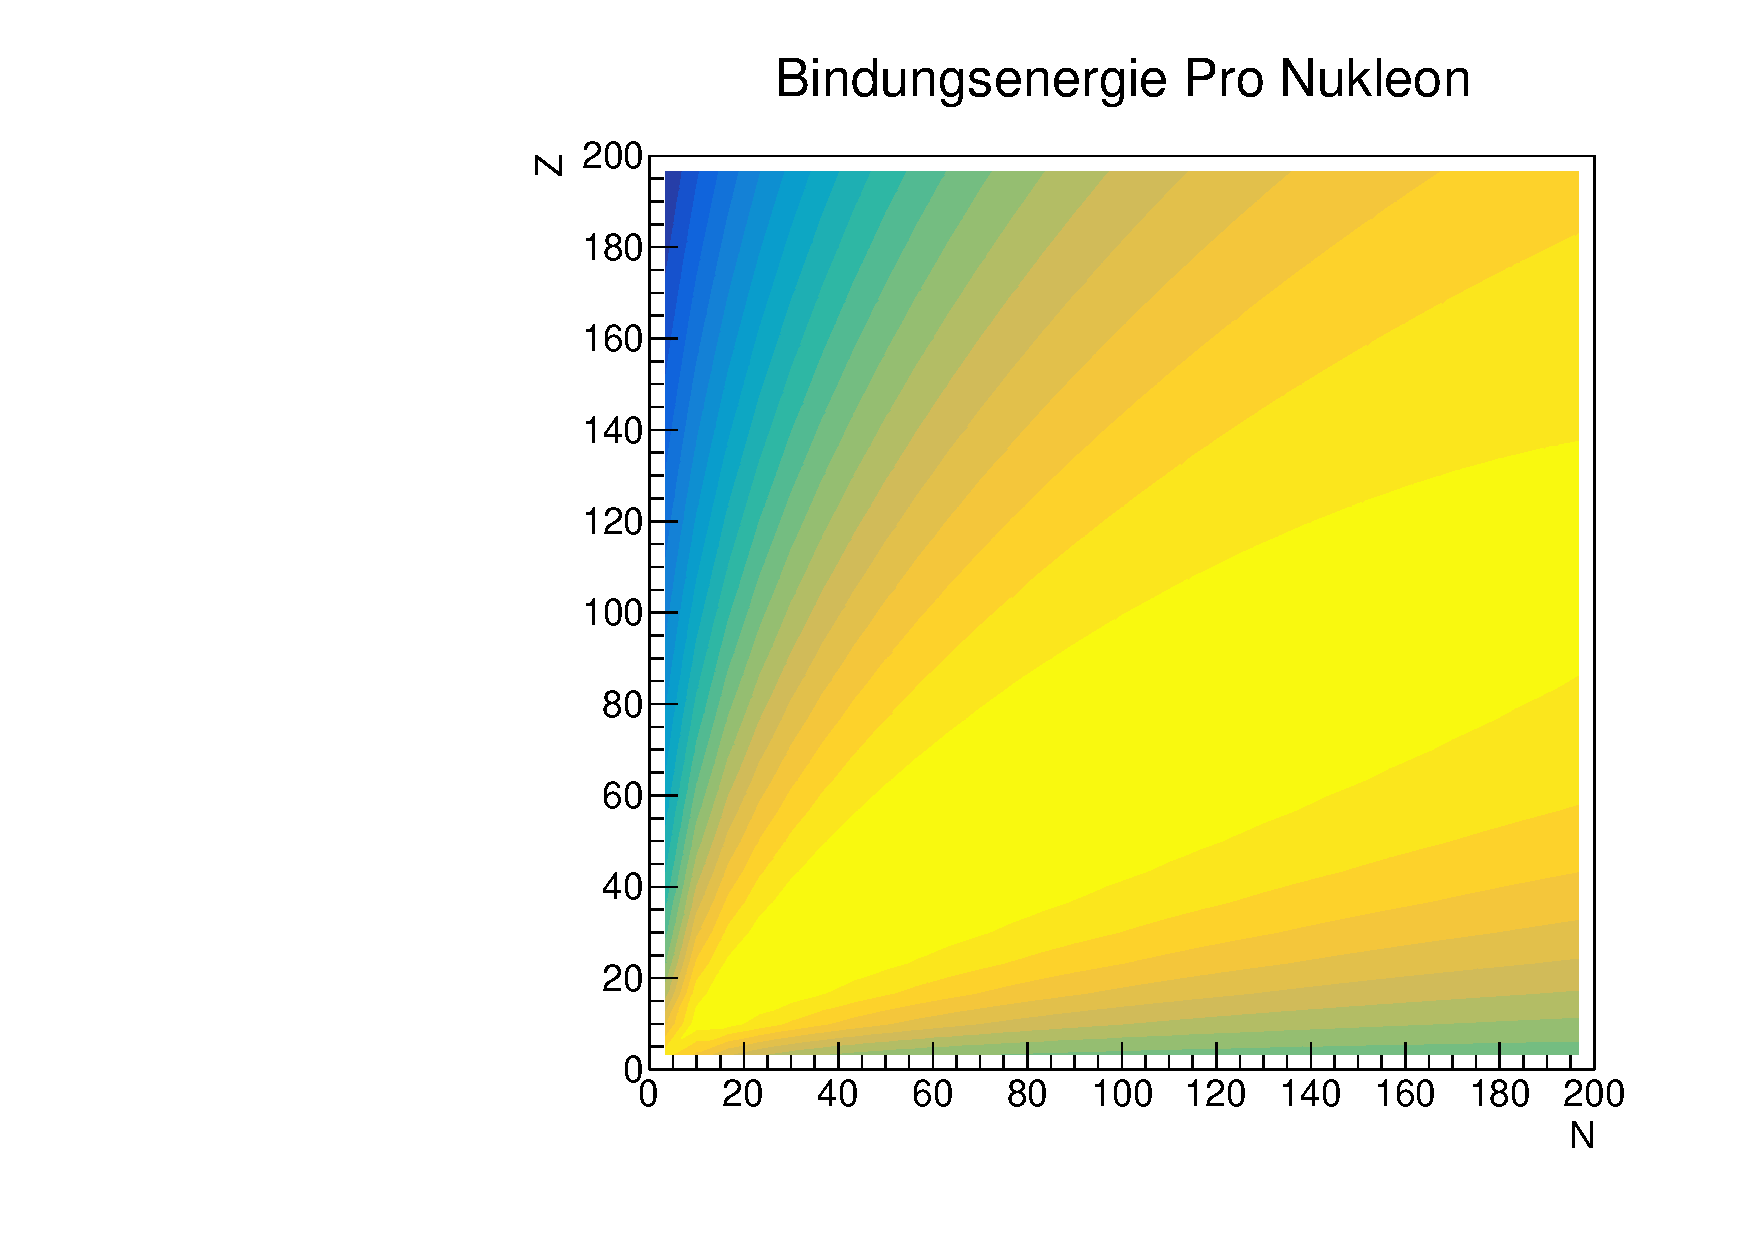
\includegraphics[width=0.6\textwidth]{figures/bindungsEnergie.pdf}
    \caption{Binding energy per nucleon using the Semi-Empirical Mass Formula. }
    \label{fig:my_label}
\end{figure}

\end{document}
